\chapter{Architectures}
\label{chp:arch}

The following chapter will show and explain the different architectures used in this thesis.
The architectures were based on existing architectures used in the automotive industry as well as experimental ones based on certain attributes.

While architectures used in the automotive industry are complex, with sometimes over 80 ECUs in one model, 
the architectures used in this thesis were sized down to a more manageable size, with ca. 20 ECUs for each architecture.
Each architecture was modeled using these components:

\begin{itemize}

    \item \textbf{ECUs}: The different ECUs in the architecture. They are the nodes of the graph.
    
    \item \textbf{Entry points}: The entry points to the architecture. The only possible entries are the external interfaces that an ECU might have.
    
    \item \textbf{Targets}: ECUs that are considered targets for an attacker. They are targets because they contain sensitive data or because they are critical for the vehicle's functionality.
    
    \item \textbf{Bus systems}: ECUs are connected to each other using bus systems. The bus systems are the edges in the graph. The possible bus systems are CAN, CANFD, LIN, FlexRay, and Ethernet.
    
    \item \textbf{Interfaces}: The interfaces are the connections between the ECUs and the external world. They are the connections between the ECUs and the bus systems. The possible interfaces are Bluetooth, WiFi, and GNSS.
    
    \item \textbf{Attack feasibility}: Each component of the architecture (ECU, bus system, interface) has its own rating for its attack feasibility.

\end{itemize}

\subsection{Components}
\label{components}

Using the scale mentioned in \ref{chp:config} for each component, a lower rating means that the component is more secure, while a higher rating means that the component is less secure.
This also indicated that the higher the overall score one architecture receives, the less secure it is.
This subsection will further explain some the aforementioned components as well as their attack feasibility based on their attributes.

    
\section{Training set architectures}
\label{sec:trainingarch}

Ten architectures were used as a "training set" to determine and calibrate the criteria used to 
evaluate the remaining architectures, which are the focus of the comparison.
This was done to avoid biasing the results, as well as have a well evaluated criteria.
In addition, the training set is much larger than the main set, thus the results are more accurate.

The following section will describe the test architectures and estimate the expected behavior of the architectures.

\subsection*{Architecture 1}
\label{sec:arch1}

\begin{figure}[h!]
    \caption{Architecture 1}
    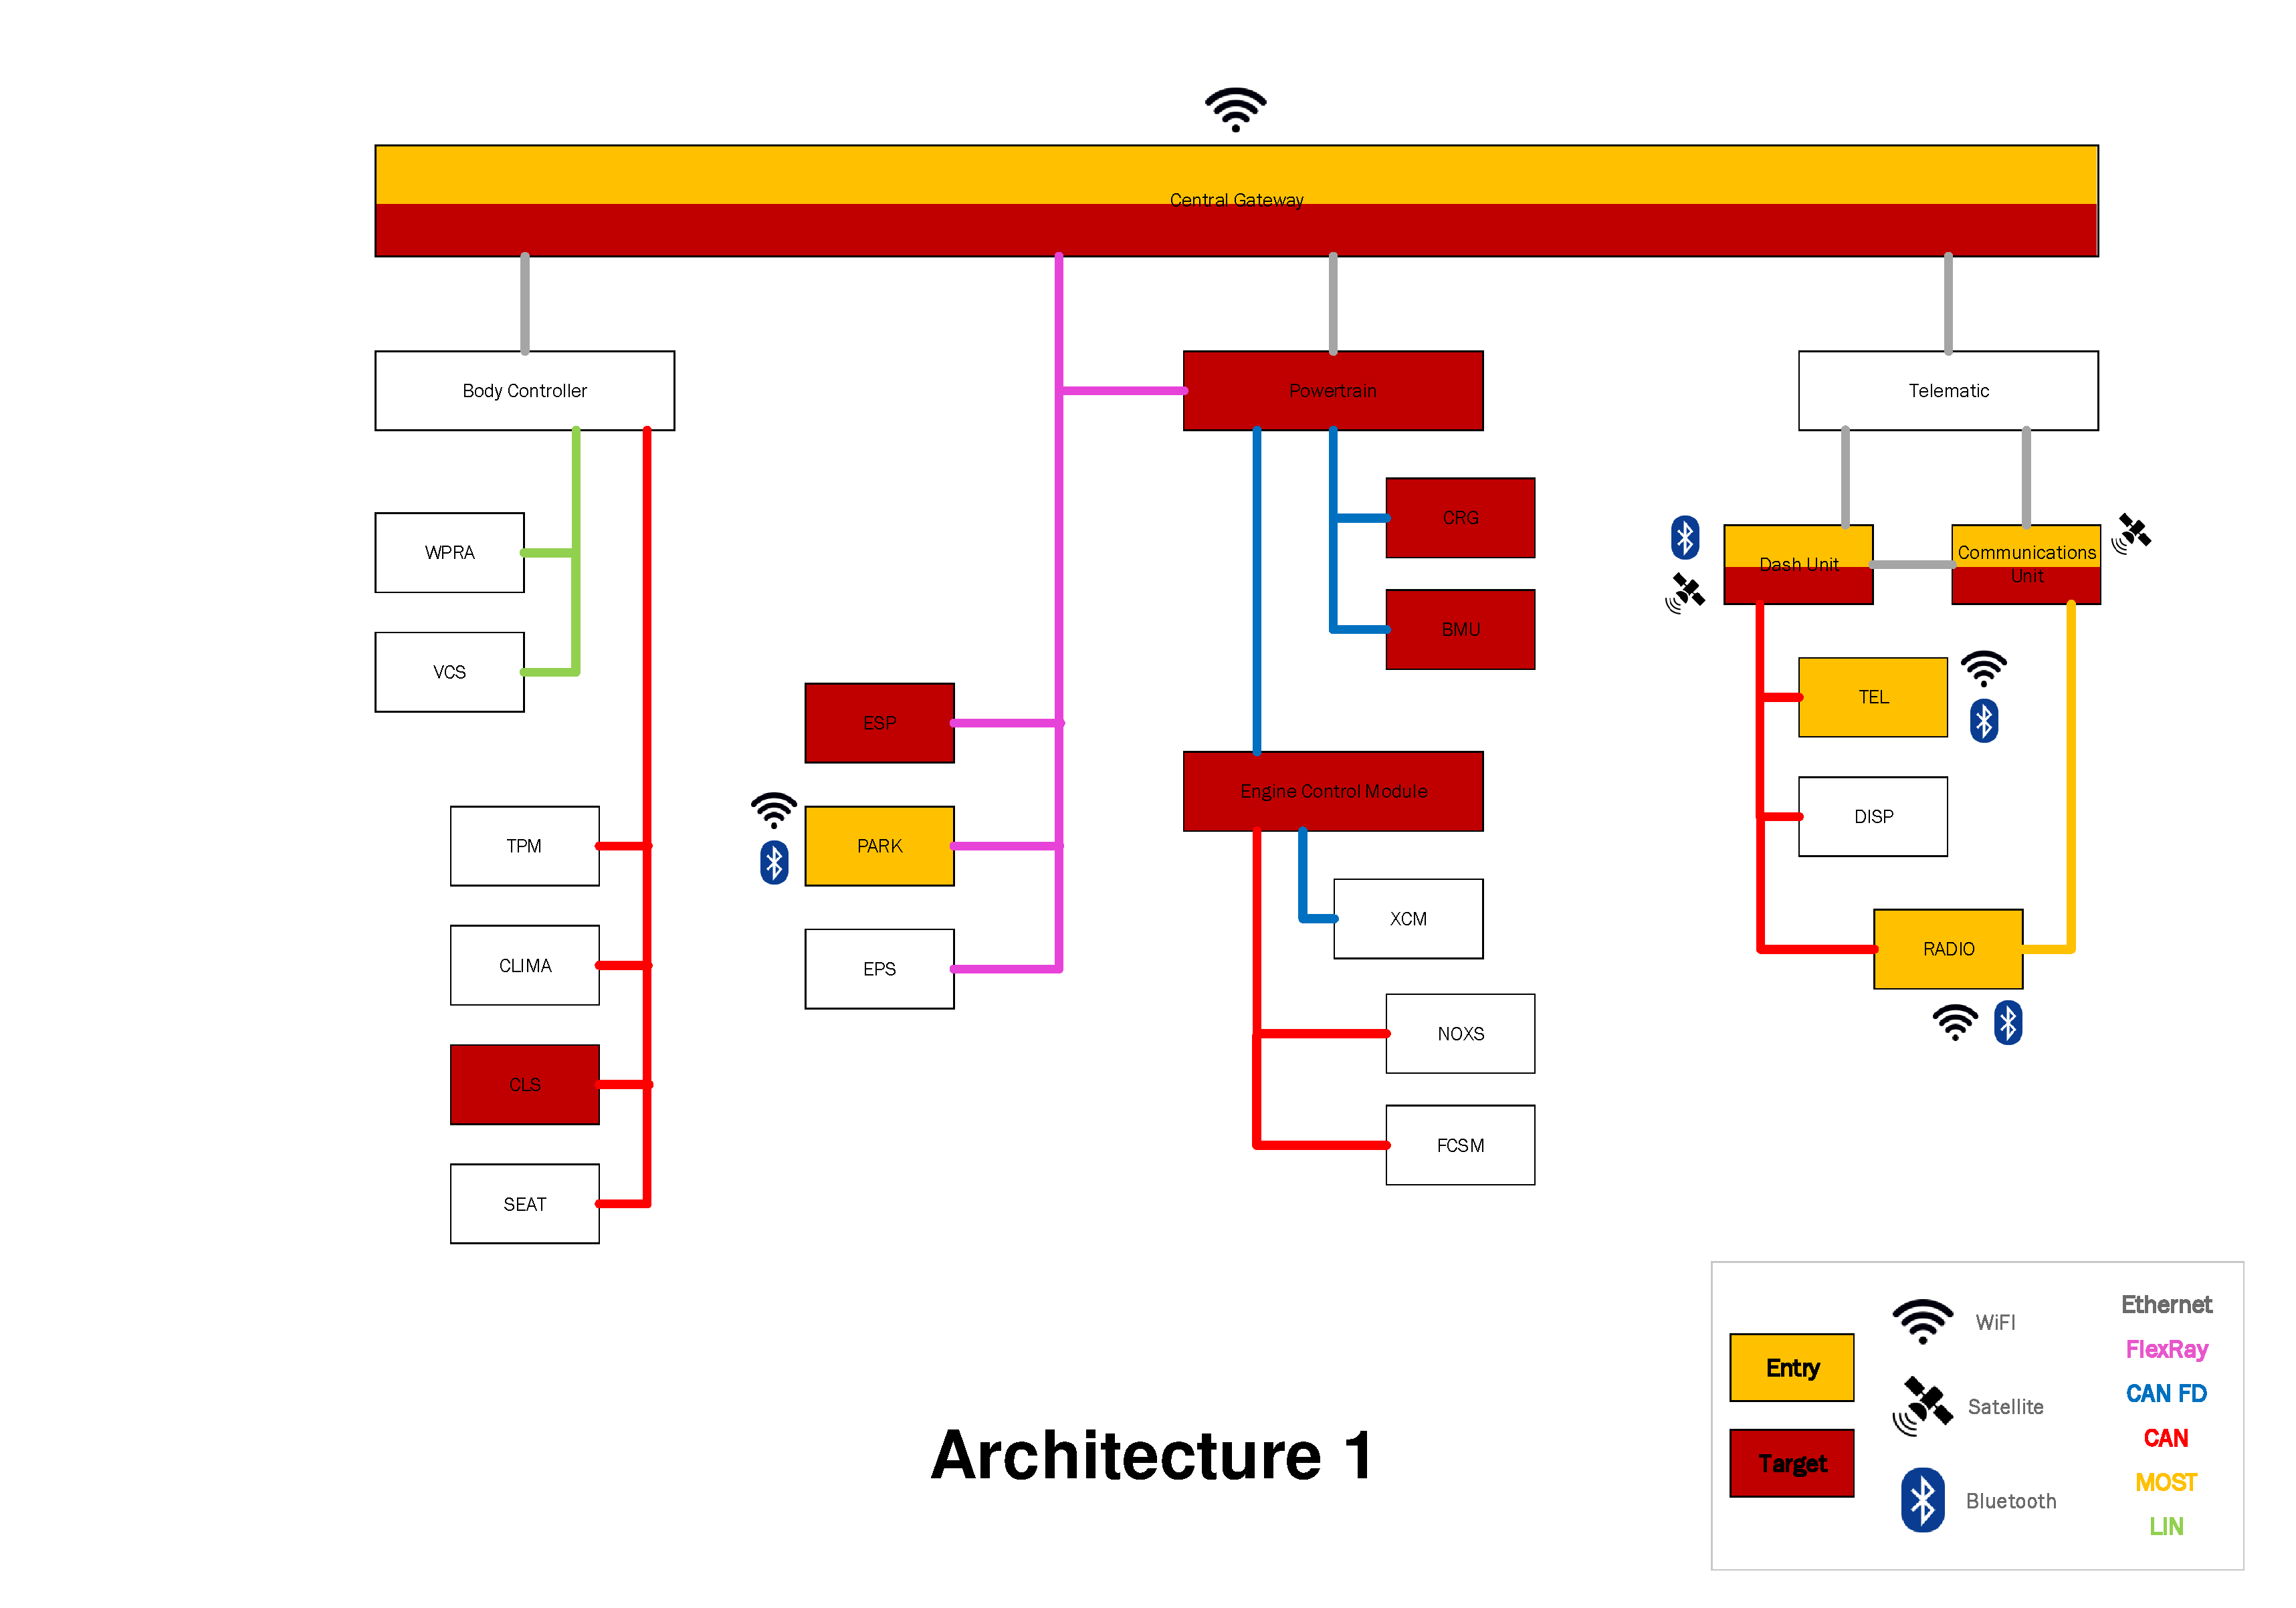
\includegraphics[width=\textwidth, page=1]{../Architectures-survey.pdf}
\end{figure}

Architecure 1 represent the most realistic architecture, as it is modeled after an actual architecture used in the automotive industry.
It was important to include this architecture, since it could offer valuable insight into the real world.
The first architecture offers six entry points with three being targets, one of it even being the \textit{Central Gateway}, and eight targets in total.
\par


\subsection*{Architecture 2}
\label{sec:arch2}	

\begin{figure}[h!]
    \caption{Architecture 2}
    \includegraphics[width=\textwidth, page=2]{../Architectures-survey.pdf}
\end{figure}

Architecure 2 is essentially the same as architecture 1, but without a central gateway, 
so we could see how the architecture would perform without it.\par


\subsection*{Architecture 3}
\label{sec:arch3}

\begin{figure}[h!]
    \caption{Architecture 3}
    \includegraphics[width=\textwidth, page=3]{../Architectures-survey.pdf}
\end{figure}

The idea of architecture 3 was to group all the entry interfaces, to see how a centralized entry would affect the architecture.
Isolating the possible entry locations reduces the attack surface, prolongs the attack path to each target, and increases the number of ECUs used for the path, thus making the attack more difficult as the attacker would have to compromise more ECUs.\par


\subsection*{Architecture 4}
\label{sec:arch4}

\begin{figure}[h!]
    \caption{Architecture 4}
    \includegraphics[width=\textwidth, page=4]{../Architectures-survey.pdf}
\end{figure}

Architecture 4 offers entry points from all domain controllers, however notice how every domain controller only has one type of interface.
In addition, ECUs that rely on more than one interface would now need to use that interface from another ECU.
For example, \textit{TEL} has to use the Bluetooth interface of the \textit{Body Controller} instead of its own Bluetooth interface.
Having an entry point from each domain controller enlargens the attack surface, as the attacker would only need to compromise one ECU in each domain controller to gain quick access to the whole domain.\par


\subsection*{Architecture 5}
\label{sec:arch5}

\begin{figure}[h!]
    \caption{Architecture 5}
    \includegraphics[width=\textwidth, page=5]{../Architectures-survey.pdf}
\end{figure}

Architecture 5 uses only Ethernet as the bus system, to see how the architecture would perform without any other bus system.
Ethernet was chosen because it recieves the securest attack feasibility rating.
In addition, there has been a trend in the automotive industry to increasingly use Ethernet as the bus system and maybe even some day replace most of the traditional CAN bus system.\par


\subsection*{Architecture 6}
\label{sec:arch6}

\begin{figure}[h!]
    \caption{Architecture 6}
    \includegraphics[width=\textwidth, page=6]{../Architectures-survey.pdf}
\end{figure}

TODO: Explain why this is interesting.
Architecture 6 puts all the ECUs onto an own bus system.
This is interesting, as the possible ECUs on a bus are limited to just one, thus many of the attack paths and number of ECUs used for the path are trimmed down to a few.
\par


\subsection*{Architecture 7}
\label{sec:arch7}

\begin{figure}[h!]
    \caption{Architecture 7}
    \includegraphics[width=\textwidth, page=7]{../Architectures-survey.pdf}
\end{figure}

TODO: Explain why this is interesting.
Architecture 7 has a similar idea to architecture 6, but instead of putting all the ECUs on their own bus system, it puts all the ECUs that used the same bus system on the same bus system.
Now, the feasibility of the bus rating is much more significant to the overall architecture rating and can indicate whether the used bus systems are secure enough.\par



\subsection*{Architecture 8}
\label{sec:arch8}

\begin{figure}[h!]
    \caption{Architecture 8}
    \includegraphics[width=\textwidth, page=8]{../Architectures-survey.pdf}
\end{figure}

Architecture 8 only has one entry point, namely the \textit{Central Gateway}. 
This architecture eliminates other entry points meaning the attack paths all start at the same point, thus reducing the attack surface.
Additionally, the feasibility rating of the interfaces is more significant than before and the attack paths might become much more linear, thus the feasibility rating of the components themselves becomes a greater factor.\par


\subsection*{Architecture 9}
\label{sec:arch9}

\begin{figure}[h!]
    \caption{Architecture 9}
    \includegraphics[width=\textwidth, page=9]{../Architectures-survey.pdf}
\end{figure}

TODO: Explain why this is interesting.
Architecture 9 is essentially the same as Architecture 4, but without a central gateway.
Again, the entry points are more dispersed resulting in an enlarged attack surface \par


\subsection*{Architecture 10}
\label{sec:arch10}

\begin{figure}[h!]
    \caption{Architecture 10}
    \includegraphics[width=\textwidth, page=10]{../Architectures-survey.pdf}
\end{figure}

TODO: Explain why this is interesting.
The final architecture of the test set only includes one of each interfaces but more dispersed than that of architecture 8.
Note that the entries are also grouped together which shares the same idea of architecture 3.\\
